\section{Showcase for the Dark QCD model}
\label{darksec}

The arguments discussed above can be illustrated using concrete BSM physics scenarios.
We will consider the ``dark'' QCD model~\cite{Bai:2013xga,Schwaller:2015gea}, which predicts 
the existence of ``emerging'' jets 
that are created in the decays of new long-lived neutral 
particles (dark hadrons), produced in a parton-shower process by dark QCD.
The process includes  two mediators of mass $M_X$ which 
decay promptly to a SM quark and a dark quark. 
The final-state signature consists of four jets with high transverse momenta, with two  
 emerging jets originating from the dark quarks.  

Searches for emerging jets have been performed in $pp$ collisions~\cite{Sirunyan:2018njd} 
by the CMS Collaboration. Such jets contain many displaced
 vertices and multiple tracks with large impact parameters, arising from the decays of the dark pions produced in the dark parton shower.
 Assuming that the mass of the dark pion is 5~GeV,  the signal acceptance using this approach does not exceed 40\% at large masses of the mediators
(see Fig.~4 of~\cite{Sirunyan:2018njd}).
The decay length of the dark pion defines the distance from the $pp$ interaction vertex 
to the point where the jet emerges. 

Alternatively, emerging jets can be reconstructed using calorimeters with high-resolution timing. This method is expected
to have advantages over the track-based method 
for the measurement of dark pions with a large decay length, i.e. in the situations where the tracker has a low
efficiency and resolution since only a few outer layers can be used for track reconstruction.
It was also pointed out~\cite{Schwaller:2015gea} that the emerging jets may have a significant fraction of neutral particles and the reconstruction
using charged tracks can have a low acceptance.

To estimate the performance of the timing layers in reconstructing emerging jets,
we use the same Monte Carlo generator settings as for Ref.~\cite{Sirunyan:2018njd}. 
The $pp$ collision event samples  were  generated with the ``hidden valley'' model framework as 
implemented in  {\sc pythia} 8.2 \cite{Sjostrand:2007gs}
assuming a centre-of-mass energy of 13~TeV and a dark pion mass of 5~GeV. 
The samples were created for different values of the decay distance $c\tau$ of the dark pions.  
The  mass $M_X$ of the mediator was also varied. 

To calculate the detector acceptance, the semi-analytical formalism based on Eq.~\ref{eqTOF} is used. In this relation $L=c\tau$ is the distance traveled
by the dark pion with mass $m$ before it decays to the emerging jet.  
We assume that such emerging jets travel to the surface of the timing layer with speed of light for all values of $m$.
This is expected since the emerging jets consist of light stable SM particles (mostly photons and pions).
  
For the timing layers, the signature of emerging jets is a time delay compared to the other SM jets. The  production vertex
cannot be observed by the timing layers if such jets emerge before TL1.
After events are generated, the weighted averages of the decay distances of all particles that originate from
the dark pions, using the particle momentum as the weight, were  calculated. This decay distance is used
to approximate the decay length, without applying a jet reconstruction algorithm.  
The  calculation for the $3\sigma$ separation assumes $m_F=m_{\alpha}\simeq 3.73$~GeV although this choice can be arbitrary.
This value of $m_F$ is used to give a conservative\footnote{One can argue that the SM jets mainly consist of light-flavour hadrons and photons, 
therefore, $m_F$ should be significantly lower.} estimate of the arrival time of the emerging SM jets.

The acceptance of the emerging jets was calculated as the fraction of  events that pass the 
Eq.~\ref{eqTOF} condition  with the parameters discussed earlier. 
 Figure~\ref{fig:efficiency_med} shows the acceptance as a function of the mediator mass $M_X$ and the decay distance
of the dark pions. This acceptance can be compared to the acceptance based on tracks~\cite{Sirunyan:2018njd}. 
The acceptance based on the TOF is significantly larger for low $M_X$ and large $L=c\tau$ of the dark pions.  
The acceptance is larger for the timing layers with a resolution better than 100~ps, as compared to the standard 1~ns resolution. 

We are interested in the acceptance  for dark pions  as a function of their mass
and lifetime assuming a fixed mass $M_X$ of the mediator. We  consider the HE-LHC environment 
with $pp$ collisions at a centre-of-mass energy of 27~TeV.    
The Monte Carlo generator settings for the signal model were similar
to those discussed in~\cite{Sirunyan:2018njd,prive}.
The mediator mass was set to 10~TeV, while the mass of the dark pion was varied in the range between 5~GeV and 1~TeV.
The dark pion decay length, $c\tau$,  was varied between 1~mm and 1000~mm, independent of its mass. Other parameters
were also appropriately modified to allow  sufficient phase space for the dark meson production.
The mass of the dark pion is assumed to be one half the mass of the dark quark. The mass of the dark
$\rho$ is four times the dark pion mass. The width of the
mediator particle is assumed to be small compared to the detector mass resolution.

As before, the acceptance for the emerging jets based on timing was calculated as the fraction of events that pass the 
Eq.~\ref{eqTOF} condition. Figure~\ref{fig:efficiency} shows the efficiency
as a function of $c\tau$ and the dark pion mass. It can be seen that a detector with the standard 1~ns resolution does
not have acceptance for the dark meson measurements. The acceptance is significantly larger when the timing layers 
 have a resolution better than 100~ps.
The acceptance is low for small $c\tau$ or small masses, which is the expected feature of the timing measurement.
The timing layers with 20~ps resolution have 100\% acceptance for large values of $c\tau$ and dark-meson masses.
The acceptance as a function of the particle velocity when using 20~ps and 1~ns resolution 
is shown in \ref{appendix}.

Note that these results are relatively general since they are formulated in terms of masses and decay lengths,  
i.e. independent of the position of the timing layers and other details relevant to 
the detector geometry.


\begin{figure}
\begin{center}
   \subfigure[10 ps] {
   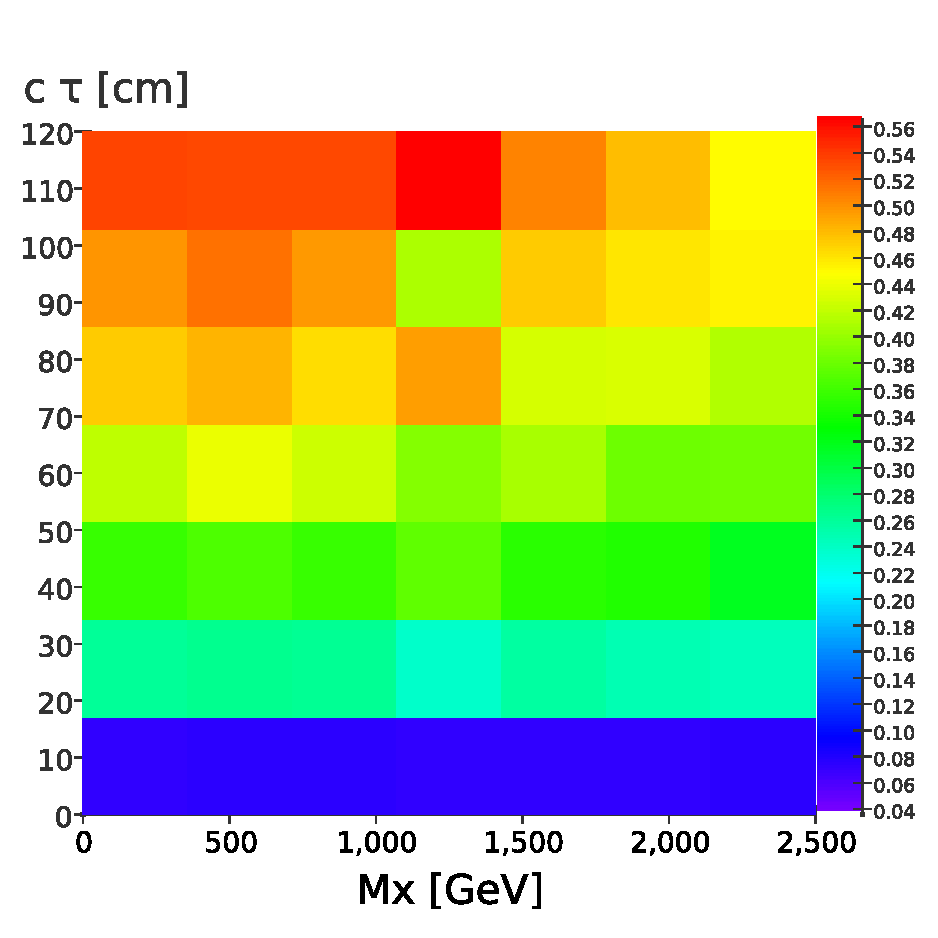
\includegraphics[width=0.39\textwidth]{effic10a_med.pdf}
   }
   \subfigure[20 ps] {
   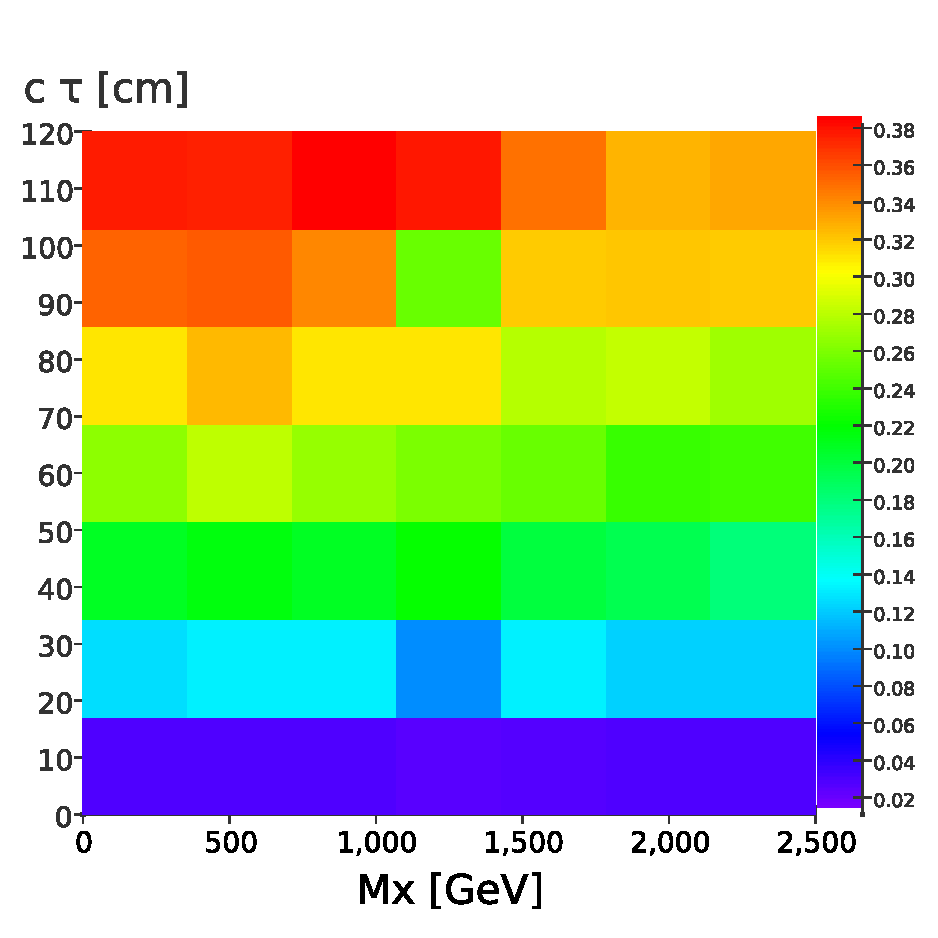
\includegraphics[width=0.39\textwidth]{effic20a_med.pdf}\hfill
   }

   \subfigure[30 ps] {
   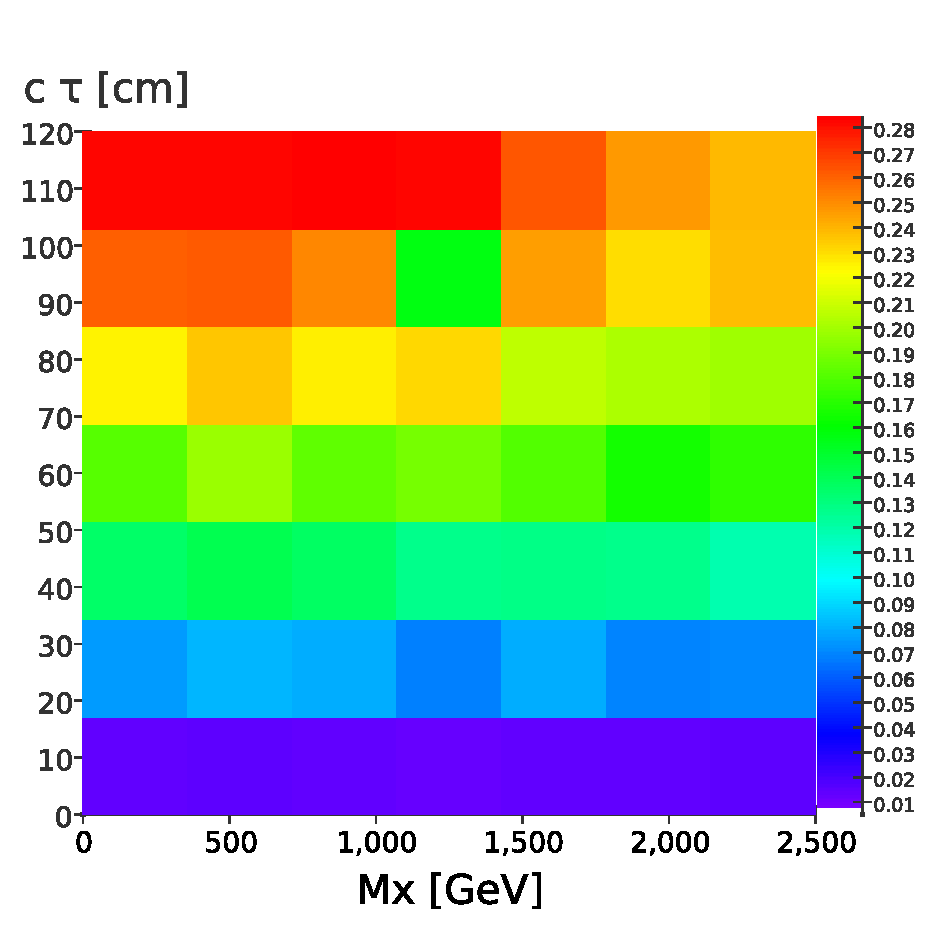
\includegraphics[width=0.39\textwidth]{effic30a_med.pdf}
   }
   \subfigure[100 ps] {
   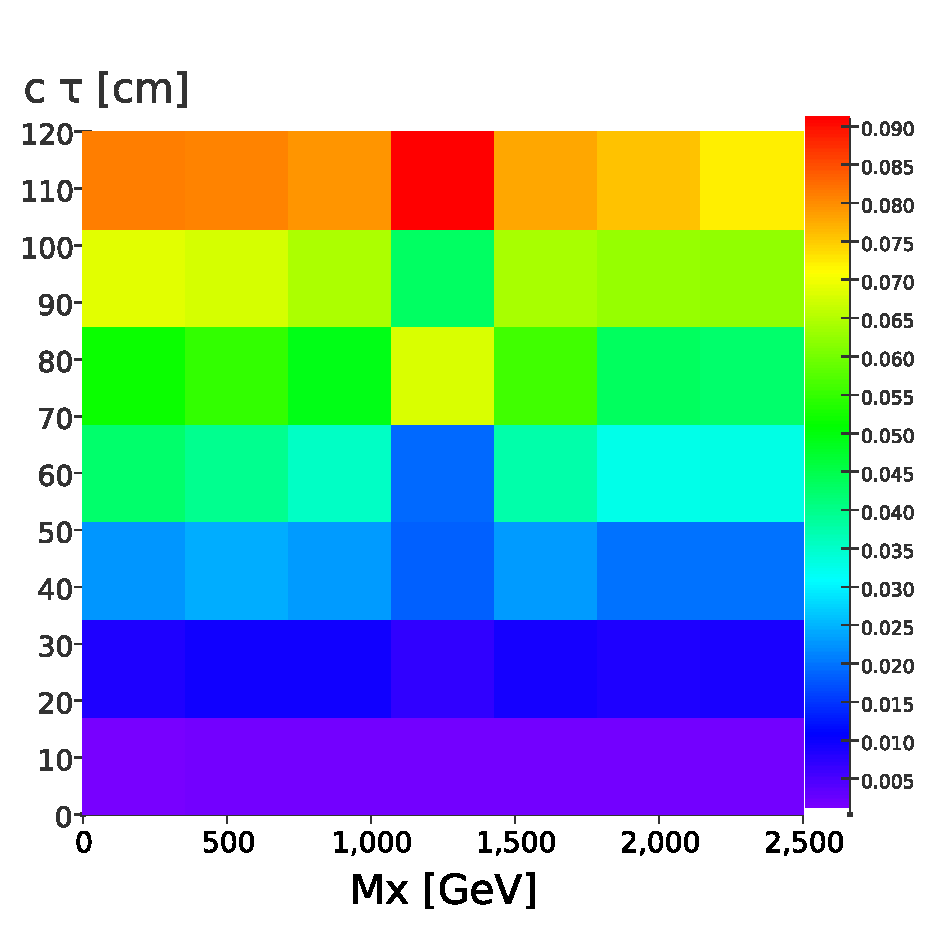
\includegraphics[width=0.39\textwidth]{effic100a_med.pdf}\hfill
   }

   \subfigure[500 ps] {
   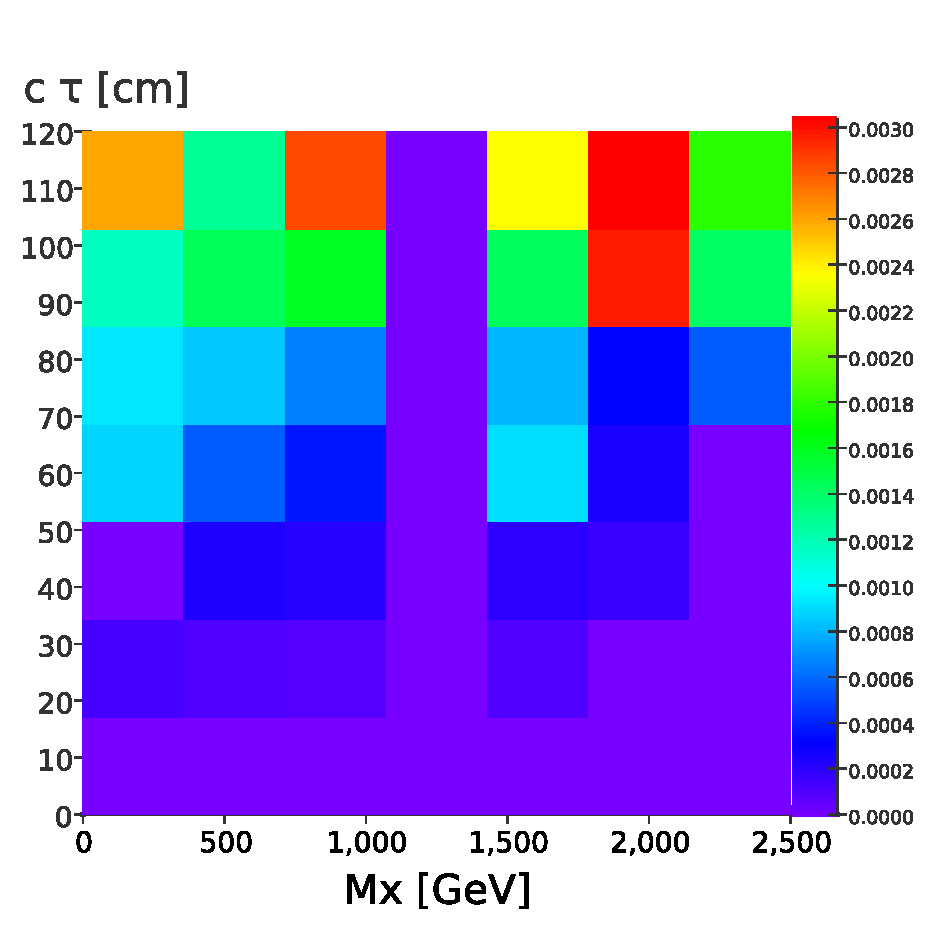
\includegraphics[width=0.39\textwidth]{effic500a_med.pdf}
   }
   \subfigure[1000 ps] {
   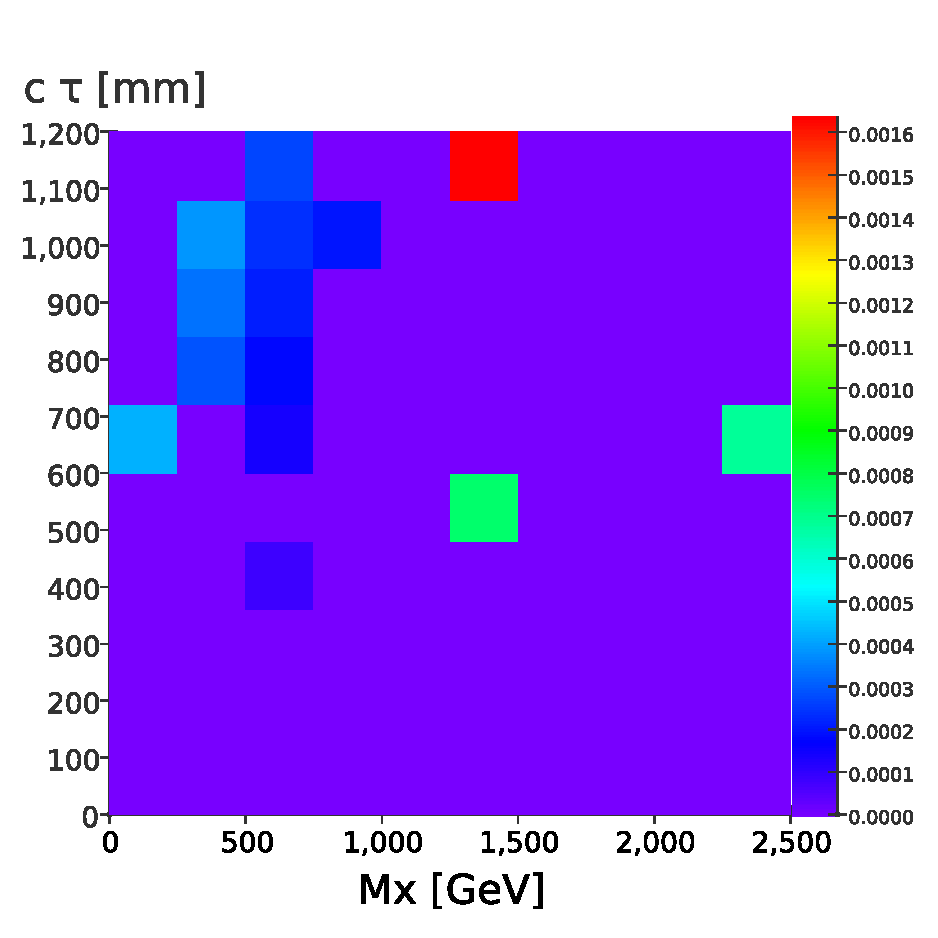
\includegraphics[width=0.39\textwidth]{effic1000a_med.pdf}\hfill
   }

\end{center}
\caption{
The acceptance for emerging jets using timing layers with different timing resolutions as
a function of the mediator mass $M_X$ and the $c\tau$ of the dark pions with mass of 5~GeV.
The {\sc pythia}8 simulations were performed
for $pp$ collisions at $\sqrt{s}=13$~TeV. The maximum values for 
the color mapping
vary from  0.56 (a)  to  0.0006 (f).  
}
\label{fig:efficiency_med}
\end{figure}

\begin{figure}
\begin{center}
   \subfigure[10 ps] {
   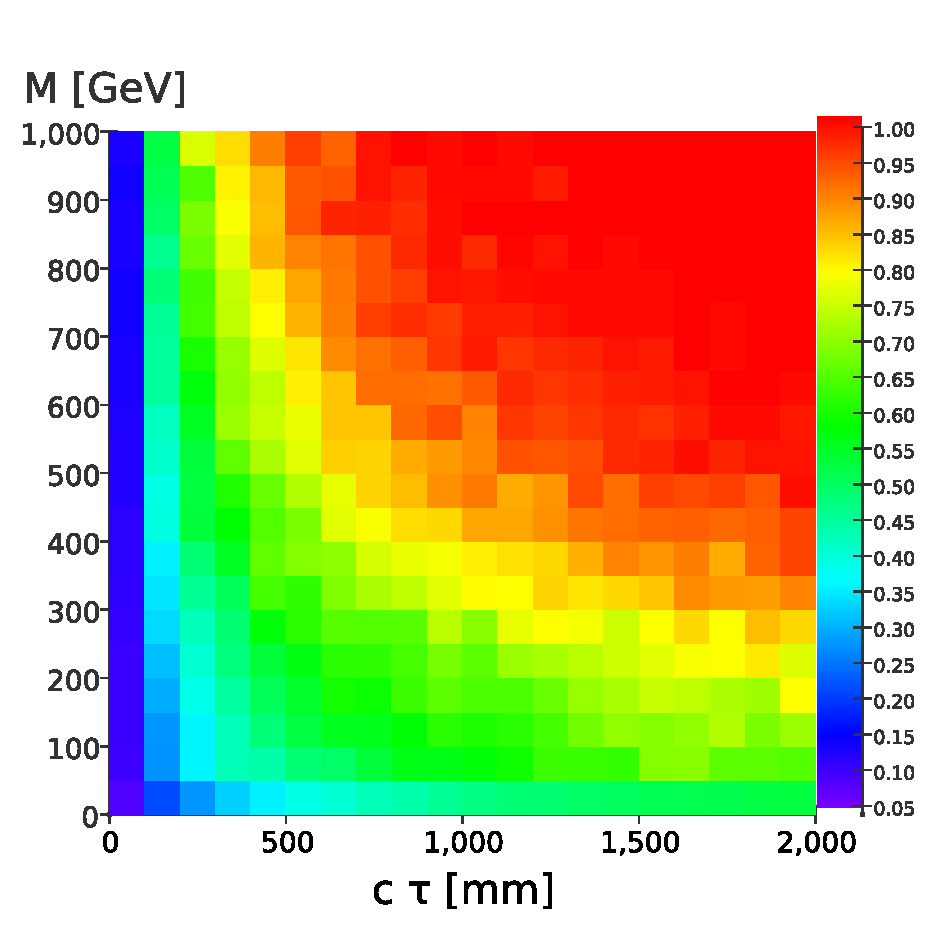
\includegraphics[width=0.39\textwidth]{effic10a.pdf}
   }
   \subfigure[20 ps] {
   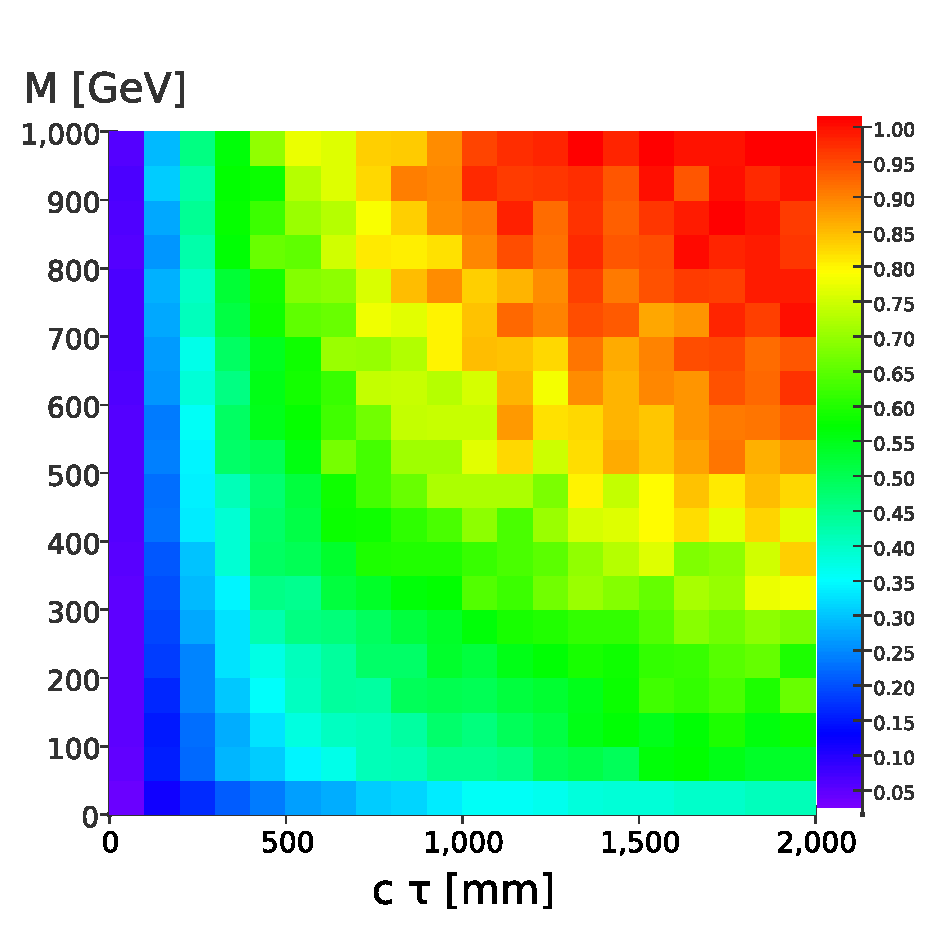
\includegraphics[width=0.39\textwidth]{effic20a.pdf}\hfill
   }

   \subfigure[30 ps] {
   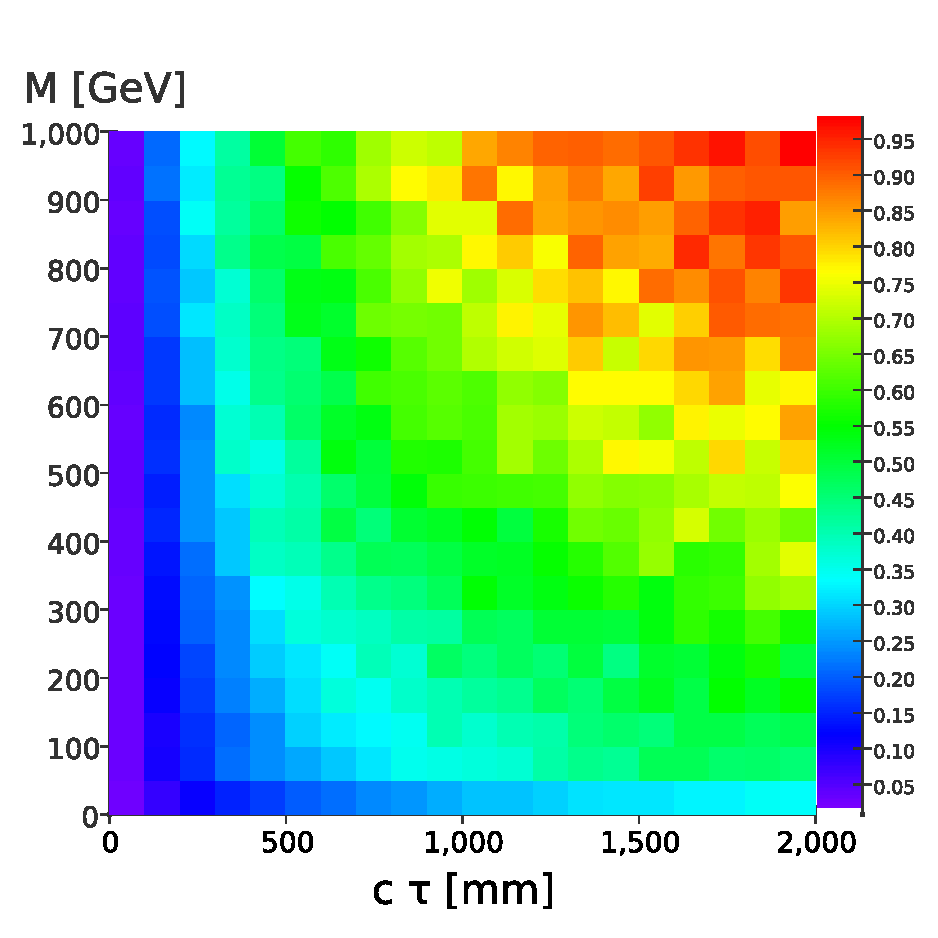
\includegraphics[width=0.39\textwidth]{effic30a.pdf}
   }
   \subfigure[100 ps] {
   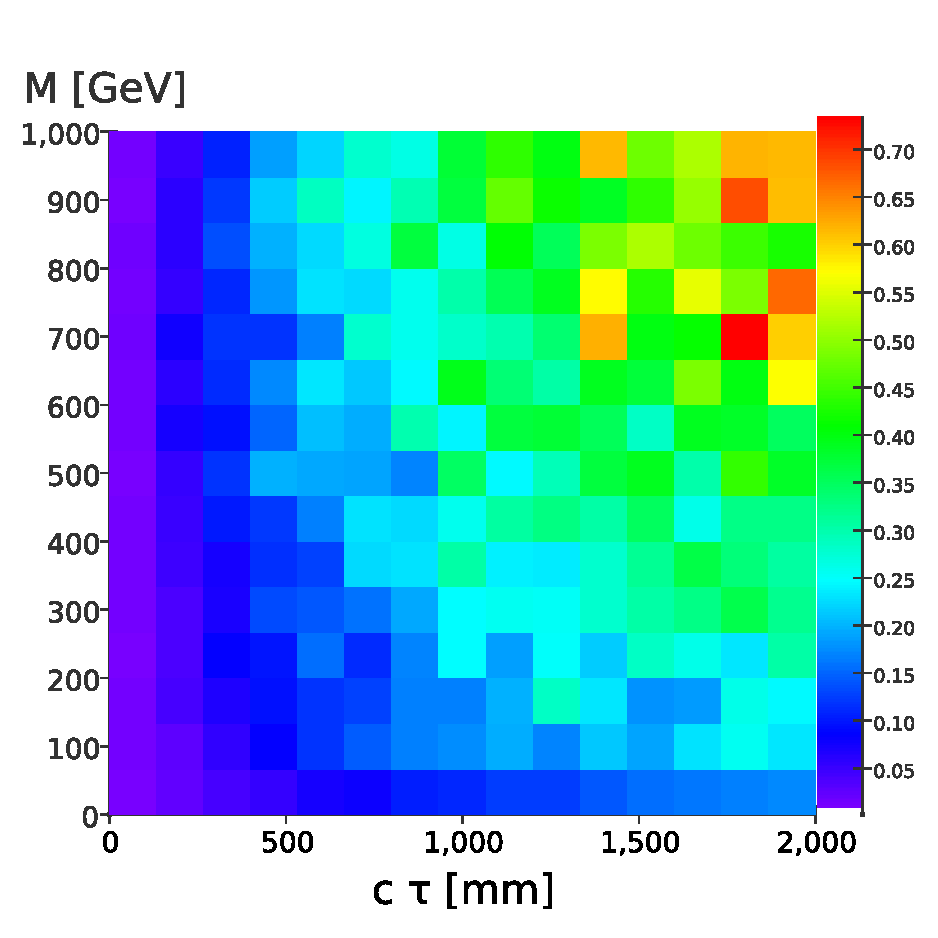
\includegraphics[width=0.39\textwidth]{effic100a.pdf}\hfill
   }

   \subfigure[500 ps] {
   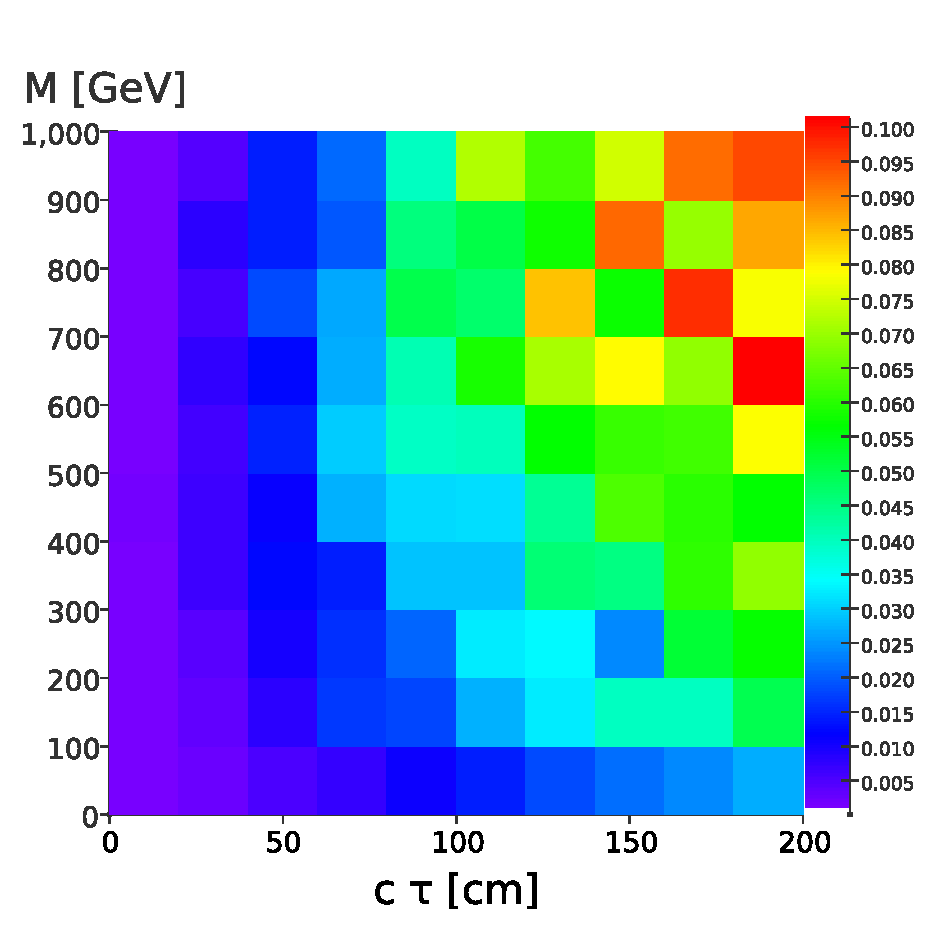
\includegraphics[width=0.39\textwidth]{effic500a.pdf}
   }
   \subfigure[1000 ps] {
   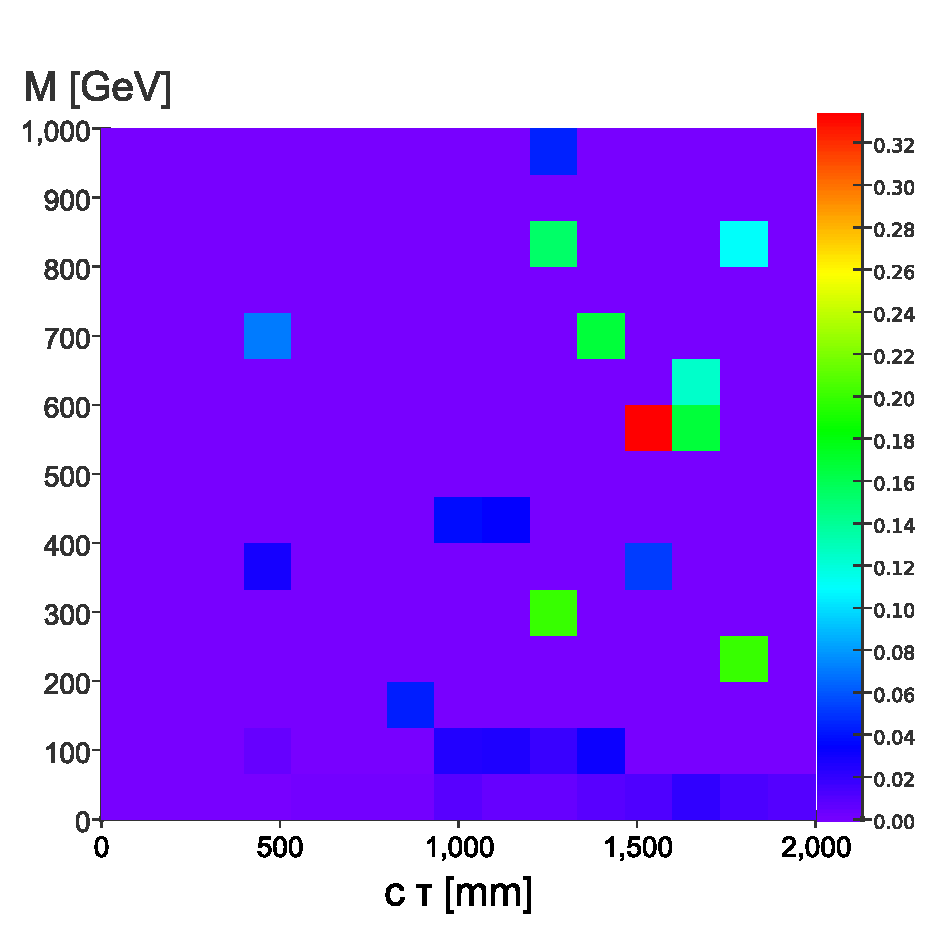
\includegraphics[width=0.39\textwidth]{effic1000a.pdf}\hfill 
   }

\end{center}
\caption{
The acceptance for emerging jets using timing layers with different timing resolutions as
a function of the dark pion mass and $c\tau$. The mediator mass was fixed at $M_X = 10$~TeV. The {\sc pythia}8 simulations were performed 
for $pp$ collisions at $\sqrt{s}=27$~TeV. 
The maximum values for 
the color mapping 
vary from  1.0 (a)  to  0.046 (f).     
}
\label{fig:efficiency}
\end{figure}

